% try to make flow chart more like diagrams in android book

\documentclass{article}
\usepackage[utf8]{inputenc}
\usepackage{tikz}
\usepackage{pgfplots}
\usetikzlibrary{shapes.geometric, arrows}

\tikzstyle{model} = [rectangle, rounded corners, minimum width=3cm, minimum height=1cm,text centered, draw=black, fill=green!30]

\tikzstyle{view} = [rectangle, rounded corners, minimum width=1cm, minimum height=1cm, text centered,  draw=black, fill=blue!30] 

\tikzstyle{process} = [rectangle, minimum width=3cm, minimum height=1cm, text centered, text width=3cm, draw=black, fill=orange!30]

\tikzstyle{decisviewn} = [diamond, minimum width=3cm, minimum height=1cm, text centered, draw=black, fill=green!30]

\tikzstyle{arrow} = [thick,->,>=stealth]

% for the legend
% argument #1: any optviewns
\newenvironment{customlegend}[1][]{%
    \begingroup
    % inits/clears the lists (which might be populated from prevviewus
    % axes):
    \csname pgfplots@init@cleared@structures\endcsname
    \pgfplotsset{#1}%
}{%
    % draws the legend:
    \csname pgfplots@createlegend\endcsname
    \endgroup
}%

% makes \addlegendimage available (typically only available within an
% axis environment):
\def\addlegendimage{\csname pgfplots@addlegendimage\endcsname}


\begin{document}

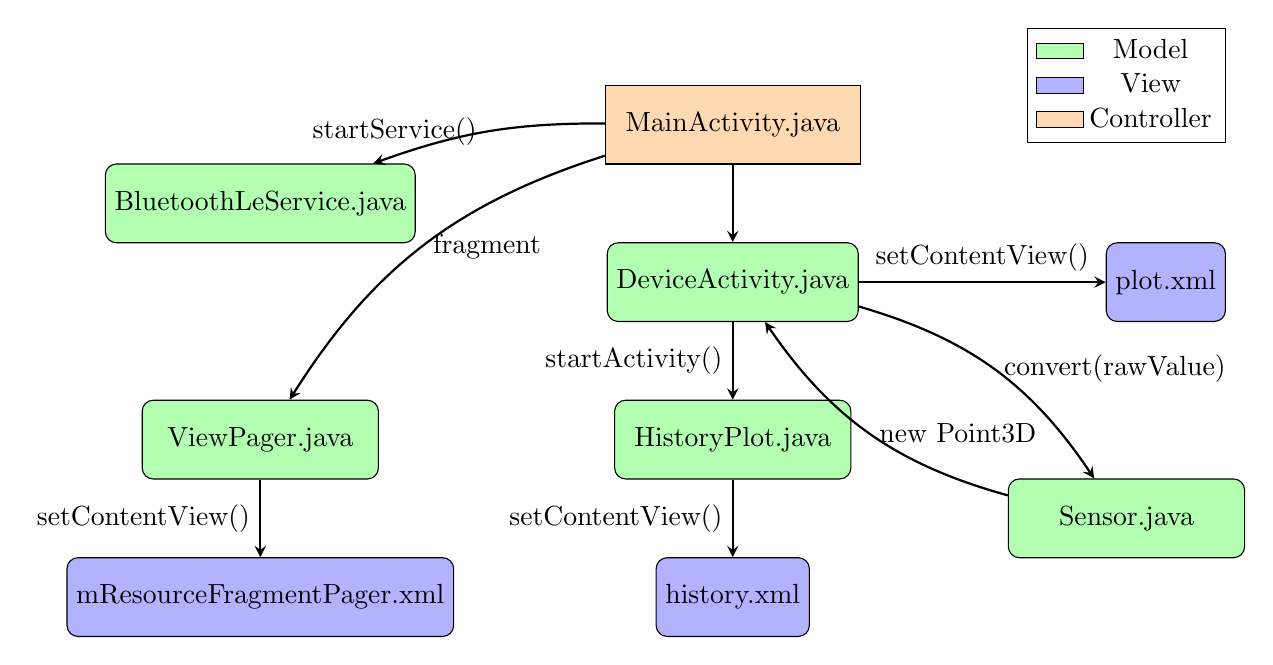
\begin{tikzpicture}[node distance=2cm]


\node (main) [process]                                     {MainActivity.java};
\node (BLE) [model, left of=main, xshift=-4cm, yshift=-1cm]{BluetoothLeService.java};

\node (DA) [model, below of=main]                          {DeviceActivity.java};
\node (plot) [view, right of=DA, xshift=3.5cm]             {plot.xml};

\node (HP) [model, below of=DA]                            {HistoryPlot.java};
\node (history) [view, below of=HP]                        {history.xml};
\node (sensor) [model, right of=HP,xshift=3cm,yshift=-1cm] {Sensor.java};

\node (VPA) [model, left of=HP, xshift=-4cm]               {ViewPager.java};
\node (fragpage) [view, below of=VPA]                      {mResourceFragmentPager.xml}; 

%% main to *
\draw [arrow] (main) to [bend right=20] node[anchor=west] {fragment} (VPA); 
\draw [arrow] (main) -- (DA);
\draw [arrow] (main) to [bend right=10] node[anchor=east] {startService()} (BLE);

% DA to * 
\draw [arrow] (DA) -- node[anchor=east] {startActivity()} (HP);
\draw [arrow] (DA) -- node[anchor=south] {setContentView()} (plot);
\draw [arrow] (DA) to [bend left=20] node[anchor=west] {convert(rawValue)} (sensor);
\draw [arrow] (sensor) to [bend left=20] node[anchor=west] {new Point3D} (DA);


\draw [arrow] (HP) -- node[anchor=east] {setContentView()} (history);

\draw [arrow] (VPA) -- node[anchor=east] {setContentView()} (fragpage);
%%\path[every node/.style={font=\sffamily\small}]

%%% second legend
%%% http://tex.stackexchange.com/questviewns/54794/using-a-pgfplots-style-legend-in-a-plain-old-tikzpicture 

\begin{customlegend}[legend entries={Model,View,Controller}, legend style={at={(5,0.5)},anchor=center}]
  \addlegendimage{black,fill=green!30,area legend}
  \addlegendimage{black,fill=blue!30,area legend}
  \addlegendimage{black,fill=orange!30,area legend}
\end{customlegend}

\end{tikzpicture}

\end{document}